\documentclass{beamer}

\usepackage{beamerthemesplit}
\usepackage[utf8x]{inputenc}
\usepackage{pgf}
\usepackage{default}
\usepackage{url}
\usepackage{subfigure}
\usepackage{algorithmic} 
\usepackage{algorithm} 
\usepackage{amssymb}
\usepackage{graphicx}
\usepackage{booktabs}

\usetheme{Singapore}


%Define some commands for printing correct variables in math mode 
\newcommand{\av}{\textbf{a}}
\newcommand{\bv}{\textbf{b}}
\newcommand{\cv}{\textbf{c}}
\newcommand{\dv}{\textbf{d}}
\newcommand{\ev}{\textbf{e}}
\newcommand{\fv}{\textbf{f}}
\newcommand{\gv}{\textbf{g}}
\newcommand{\hv}{\textbf{h}}
\newcommand{\iv}{\textbf{i}}
\newcommand{\jv}{\textbf{j}}
\newcommand{\kv}{\textbf{k}}
\newcommand{\lv}{\textbf{l}}
\newcommand{\mv}{\textbf{m}}
\newcommand{\nv}{\textbf{n}}
\newcommand{\ov}{\textbf{o}}
\newcommand{\pv}{\textbf{p}}
\newcommand{\qv}{\textbf{q}}
\newcommand{\rv}{\textbf{r}}
\newcommand{\sv}{\textbf{s}}
\newcommand{\tv}{\textbf{t}}
\newcommand{\uv}{\textbf{u}}
\newcommand{\vv}{\textbf{v}}
\newcommand{\wv}{\textbf{w}}
\newcommand{\xv}{\textbf{x}}
\newcommand{\yv}{\textbf{y}}
\newcommand{\zv}{\textbf{z}}

\newcommand{\alphav}{\mbox{\boldmath$\alpha$}}
\newcommand{\betav}{\mbox{\boldmath$\beta$}}
\newcommand{\gammav}{\mbox{\boldmath$\gamma$}}
\newcommand{\xiv }{\mbox{\boldmath$\xi$}}
\newcommand{\muv}{\mbox{\boldmath$\mu$}}
\newcommand{\tauv}{\mbox{\boldmath$\tau$}}
\newcommand{\Omegam}{\mbox{\boldmath$\Omega$}}
\newcommand{\Lambdam}{\mbox{\boldmath$\Lambda$}}
\newcommand{\Sigmam}{\mbox{\boldmath$\Sigma$}}
\newcommand{\Gammam}{\mbox{\boldmath$\Gamma$}}
\newcommand{\Deltam}{\mbox{\boldmath$\Delta$}}
\newcommand{\Thetam}{\mbox{\boldmath$\Theta$}}
\newcommand{\Phim}{\mbox{\boldmath$\Phi$}}
\newcommand{\Pim}{\mbox{\boldmath$\Pi$}}

\newcommand{\diag}{\mbox{diag}}
\newcommand{\tr}{\mbox{tr}}
\newcommand{\card}{\mbox{card}}
\newcommand{\cov}{\mbox{cov}}
\newcommand{\sign}{\mbox{sign}}
\newcommand{\var}{\mbox{var}}
\newcommand{\st}{\mbox{s.t.}}
\newcommand{\rank}{\mbox{rank}}
\newcommand{\argmin}{\mbox{argmin}}
\newcommand{\argmax}{\mbox{argmax}}

\newcommand{\Am}{\textbf{A}}
\newcommand{\Bm}{\textbf{B}}
\newcommand{\Cm}{\textbf{C}}
\newcommand{\Dm}{\textbf{D}}
\newcommand{\Em}{\textbf{E}}
\newcommand{\Fm}{\textbf{F}}
\newcommand{\Gm}{\textbf{G}}
\newcommand{\Hm}{\textbf{H}}
\newcommand{\Imat}{\textbf{I}}
\newcommand{\Jm}{\textbf{J}}
\newcommand{\Km}{\textbf{K}}
\newcommand{\Lm}{\textbf{L}}
\newcommand{\Mm}{\textbf{M}}
\newcommand{\Nm}{\textbf{N}}
\newcommand{\Om}{\textbf{O}}
\newcommand{\Pm}{\textbf{P}}
\newcommand{\Qm}{\textbf{Q}}
\newcommand{\Rm}{\textbf{R}}
\newcommand{\Sm}{\textbf{S}}
\newcommand{\Tm}{\textbf{T}}
\newcommand{\Um}{\textbf{U}}
\newcommand{\Vm}{\textbf{V}}
\newcommand{\Wm}{\textbf{W}}
\newcommand{\Xm}{\textbf{X}}
\newcommand{\Ym}{\textbf{Y}}
\newcommand{\Zm}{\textbf{Z}}

%Use regular expression: (\[a-z])([^a-zA-Z])  -> \1v\2  to change old style macros 
\graphicspath{{./Figures/}}

\title{Statistics and the Analysis of Data\\ Lecture 3: An Introduction to Probability Theory}
\author{Charanpal Dhanjal \\ \texttt{charanpal@gmail.com}} 
\institute{\'{E}cole des Ponts}
\date{5th November 2013}

\begin{document}

\frame{\titlepage}


\begin{frame}{Recap Part I}  
\begin{itemize} 
\item PCA is method to deal with multivariate data 
\item Represent observations in matrix form 
\begin{displaymath} 
 \textbf{X} = \left[\begin{array}{c c c} x_{11} & \ldots & x_{1d} \\ 
                     \vdots & \ddots & \vdots \\
 x_{n1} & \ldots & x_{nd}  \end{array} \right]  = \left[\begin{array}{c} \xv_1^T \\ \vdots \\  \xv_n^T \end{array} \right]
\end{displaymath}
\item PCA forms a linear combination of columns of $\textbf{X}$ that are uncorrelated (``hidden'' variables)
\end{itemize}
\end{frame}


\begin{frame}{Recap Part II}
\begin{itemize} 
 \item First we must centre and normalise data 
\item We want a $k$ dimensional projection that captures most variance such that $\Vm^T\Vm = \Imat$
 \begin{displaymath}
  \max \phi(\Vm) = \max \sum_{i=1}^n \|\xv_{i}^T\Vm\Vm^T \|^2
 \end{displaymath}
\end{itemize}
\end{frame}

\begin{frame}{Recap Part III} 
Best orthogonal $\Vm$ which maximises variance 
  \begin{figure}[htp]
\mbox{
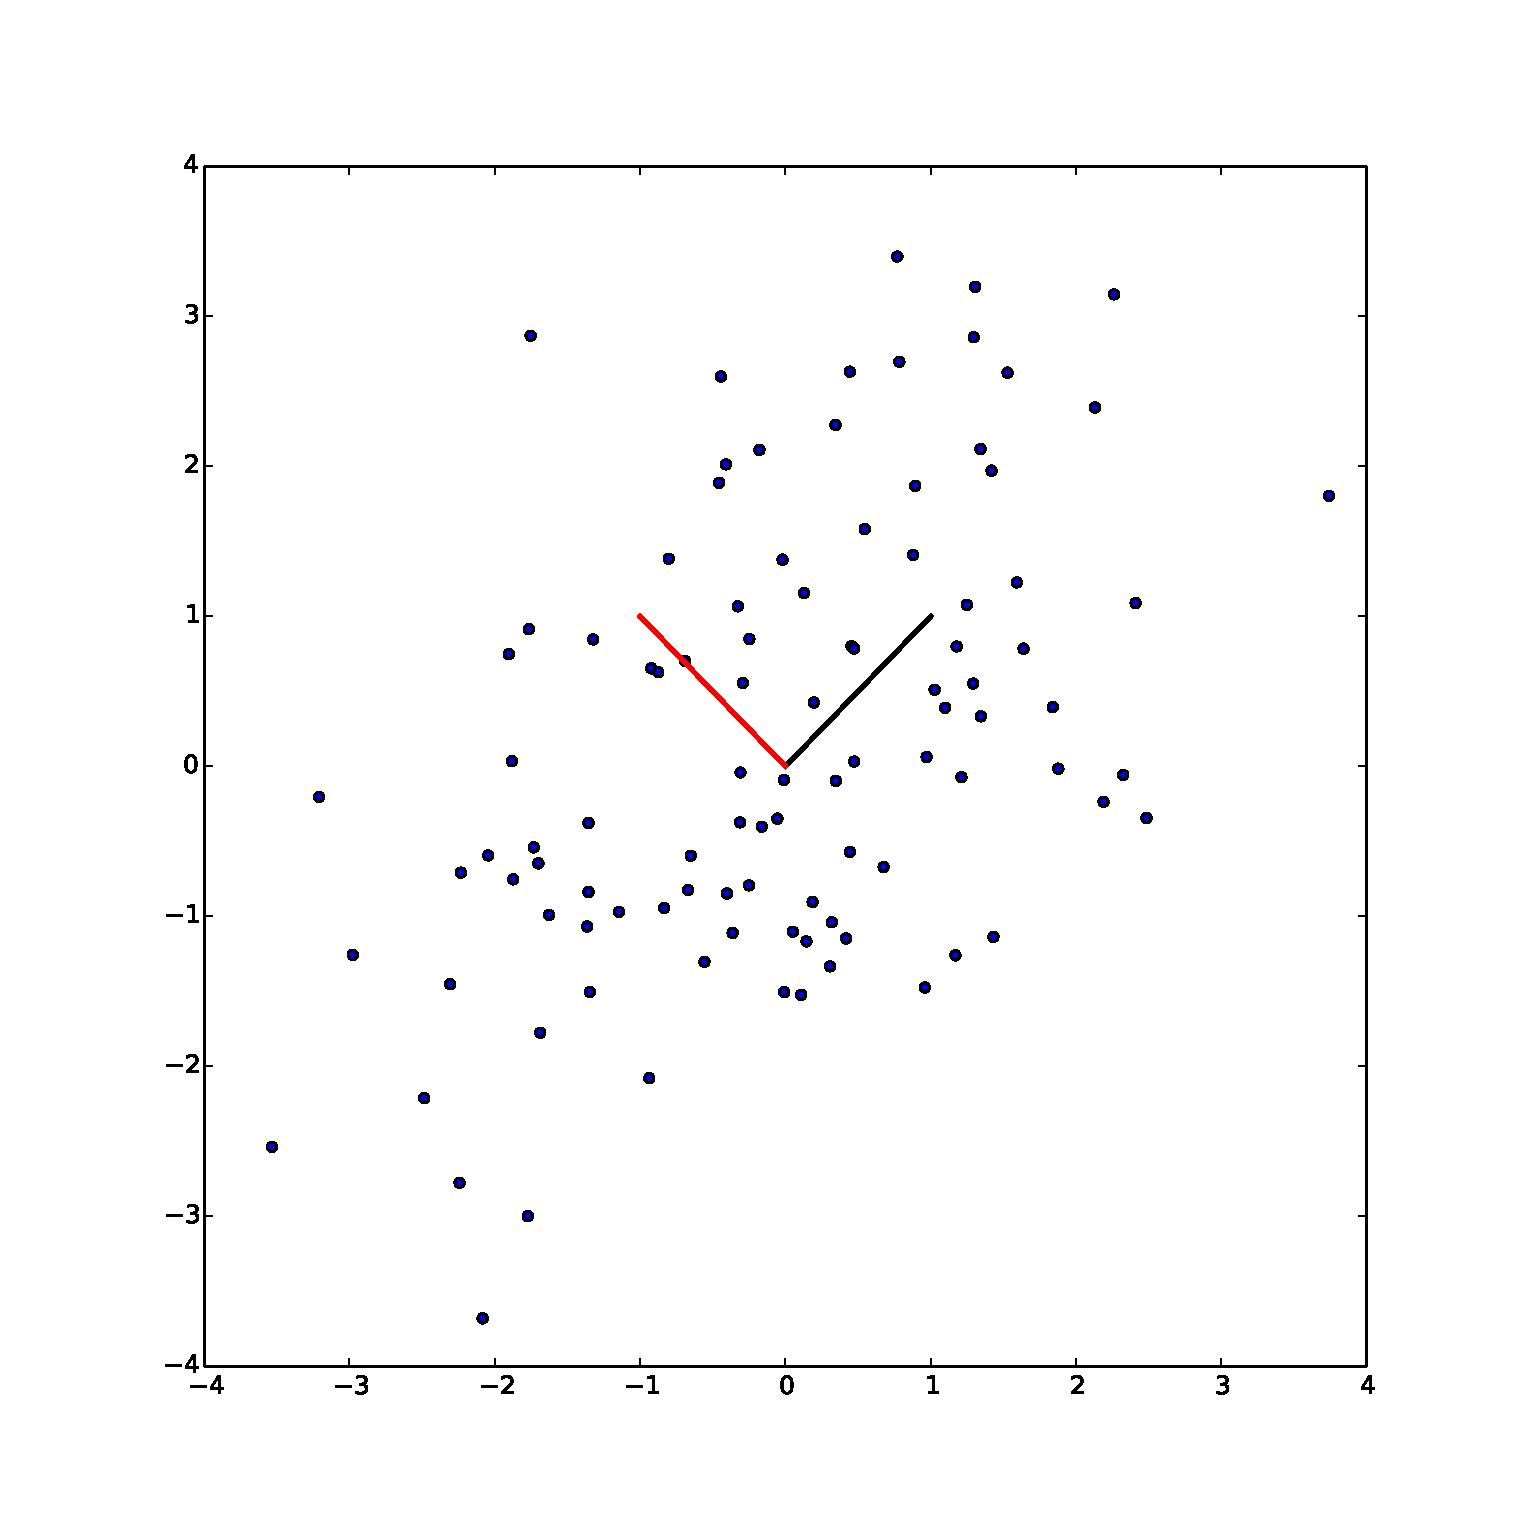
\includegraphics[width=0.5\linewidth]{PCA.eps}
}
\end{figure} 
\end{frame}

\begin{frame}{Recap Part IV} 
\begin{itemize} 
 \item To solve this find the eigenvectors (denote by columns of $\Vm$) corresponding to largest eigenvalues of covariance matrix $\Cm = \frac{1}{n}\Xm^T\Xm$ 
 \item New features are $\Zm = \Xm\Vm$, known as \emph{Principal Components}
\end{itemize}
\end{frame}


\begin{frame}{Motivations}
\begin{itemize} 
 \item Probabilities are everywhere 
 \begin{itemize}
 \item Games
 \item Passing genes from parent to child 
 \item Medical trials
 \item Behaviour of groups of people 
 \end{itemize} 
\item These events can be modelled 
\item Applications: search engines, insurance, energy demand prediction etc. 
\end{itemize}
\end{frame}

\begin{frame}{What is Probability?} 
\begin{itemize}
 \item Repeated tosses of a coin give unpredictable results. 
 \item Some terminology 
 \begin{itemize}
 \item An \emph{experiment} gives us an observation of the random event
 \item The \emph{sample space} $S$ is the set of all outcomes of an experiment e.g. $S = \{H, T\}$ for coin toss, $S = \{1,2,3,4,5,6\}$ for a die  
 \item By \emph{event} we mean some $E \subseteq S$ 
 \end{itemize} 
 \item To find the probability of an event we repeat the same experiment approaching an infinite number of times 
 \item Sometimes even large numbers of experiments are difficult e.g. firearms ban on gun crime,  austerity/stimulus on recessions 
\end{itemize}
\end{frame}

\begin{frame}{Definitions}
\begin{itemize}
 \item Let $A \subseteq S$ then the probability of $A$ occurring is denoted by $P(A) \in [0, 1]$
 \item Some properties 
 \begin{itemize}
 \item $P(\emptyset) = 0$
 \item $P(S) = 1$
 \item $P(A^c) = 1 - P(A) \quad \forall A$,  where $A^c = S \backslash A$
 \item Let $A_1, A_2, \ldots, A_k$ be disjoint sets i.e. $A_i \cap A_j = \emptyset, i \neq j$, then 
 \begin{displaymath} 
  P\left(\bigcup_{i=1}^k A_i \right) = \sum_{i=1}^k P(A_i)
 \end{displaymath}
 \end{itemize} 
\end{itemize}
\end{frame}

\begin{frame}{An Example} 
\begin{itemize} 
 \item Imagine throwing a die with 6 faces, $S = \{1,2,3,4,5,6\}$
\item Assuming die is fair $P(\{a\}) = 1/6$ for $a = 1, \ldots, 6$
\item What is the probability of throwing a numbers less than or equal to 2? $P(\{1\}) = 1/6, P(\{2\}) = 1/6 \Rightarrow P(\{1, 2\}) = 1/3$
\end{itemize}
\end{frame}

\begin{frame}{More Definitions}  
\begin{itemize}
 \item A \emph{complementary event} is given by $A^c = S \backslash A$ 
\item A certain event is given by $S$ and an impossible one is $\emptyset$
\item Union of events $A \cup B$ when either $A$ occurs or $B$ occurs
\item The intersection of events $A \cap B$ occurs when $A$  and $B$ occur
\item Two events are \emph{exclusive} when $A \cap B = \emptyset$ 
\item \emph{Elementary events} contain a single element $A = \{a\}, a \in S$ 
\end{itemize} 
\end{frame}

\begin{frame}{Examples} 
\begin{itemize} 
 \item Consider again a die
\begin{itemize}
\item If $A$ is the set of even numbers then $A^c$ the set of odd ones
\item The outcome of a throw is positive is a certain event 
\item The outcome is greater than 6 is an impossible event 
\item The union of odd and even numbers is a certain event 
\item The intersection of even numbers and numbers divisible by 3 is the event ${6}$
\end{itemize}
 \end{itemize}
\end{frame}

\begin{frame}{Independence} 
\begin{itemize}
 \item Two events $A$ and $B$ are independent if 
\begin{displaymath} 
 P(A \cap B) = P(A)P(B)
\end{displaymath}
\item Consider two dice with events $A$ being the 1st is even, and $B$ being the 2nd is 1
\begin{itemize}
\item $P(A) = \sum_{i=1}^3 \sum_{j=1}^6 P(\{2i, j\}) = 18 \times \frac{1}{36} = \frac{1}{2}$
\item $P(B) =  \sum_{i=1}^6 P(\{i, 1\}) = 6 \times \frac{1}{36} = \frac{1}{6}$
\item $P(A \cap B) = \sum_{i=1}^3 P(\{2i, 1\}) = 3 \times \frac{1}{36}  = \frac{1}{12}$ 
\item $\Rightarrow$ $A$, $B$ independent 
\end{itemize}
\end{itemize}
\end{frame}

\begin{frame}{Another Example}  
 \begin{itemize}
  \item We throw a die and let $A$ be the event that the outcome is even and $B$ that it is a multiple of 3
\begin{itemize}
\item $P(A) = \sum_{i=1}^3 P(\{2i\}) = 3 \times \frac{1}{6} = \frac{1}{2}$ 
\item $P(B) = \sum_{i=1}^2 P(\{3i\}) = 2 \times \frac{1}{6} = \frac{1}{3}$ 
\item $P(A \cap B) = P(\{6\}) = \frac{1}{6}$ 
\item So these events are independent 
 \end{itemize}
 \end{itemize}
\end{frame}


\begin{frame}{Exercise}
\begin{itemize} 
 \item In the previous example, are events still independent if $P(\{2\}) = 0$ and $P(\{6\}) = 1/3$? 
 \item Consider a room of $n$ people. What is the smallest $n$ such that at least two have the same birthday with probability $> 0.5$? 
 \begin{itemize} 
 \item Assume there are no leap years, and birthdays fall on all days with equal probability  
 \item Note: it is not required to find the correct $n$, but suggest an efficient computational way to find it. 
 \end{itemize}
\end{itemize}
\end{frame}

\begin{frame}{Conditional Probabilities}
\begin{itemize} 
 \item The probability of an event can change if another event occurs. e.g. the probability of having a hard disk failing increases if its age is greater than 5 years. 
\item Let $A$ and $B$ be two events. Then the \emph{conditional probability} of $A$ given $B$ where $P(B) \neq 0$ is: 
\begin{displaymath} 
 P(A | B) = \frac{P(A \cap B)}{P(B)}
\end{displaymath}
\item Properties 
\begin{itemize}
\item $P(A | A) = 1$
\item $P(A | B) = P(A)$ iff $A$ and $B$ are independent 
\end{itemize}
\end{itemize} 
\end{frame}

\begin{frame}{Bayes' Law} 
\begin{itemize}
 \item We can write for a partition of the sample space $A_1, \ldots, A_n$: 
\begin{displaymath}
 P(B) = \sum_{i=1}^n P(B | A_i) P(A_i)
\end{displaymath}
\item Bayes' Law says for $P(B)>0$: 
\begin{displaymath}
 P(A | B) = \frac{P(B | A)P(A)}{P(B)}
\end{displaymath}
where $P(A)$ is the \emph{prior} (initial belief in $A$), $P(A|B)$ is the \emph{posterior} (belief in $A$ given $B$), and $P(B | A)$ is called \emph{likelihood} 
\end{itemize}
\end{frame}

\begin{frame}{Exercise} 
 \begin{itemize} 
  \item At a petrol station, 35\% buy leaded petrol, 40\% buy unleaded and 25\% buy super-unleaded. The respective proportions who fill their tanks are 60\%, 30\%, 50\%. Calculate the following probabilities 
\begin{itemize}
\item  The next client will fill their tank and use unleaded petrol 
\item The next client will fill their tank. 
\item Assuming the client fills their tank, what is the probability they buy leaded petrol. 
\end{itemize}
 \end{itemize}
\end{frame}

\begin{frame}{Summary}
 \begin{itemize} 
  \item Probabilities, events, sample space  
  \item Conditional independence
  \item Bayes' Law 
 \end{itemize}

\end{frame}


\end{document}